\subsection{Brief Design Specification}
\subsubsection{Overall summary description of the module}
This module should function as a calculator and be designed by ourselves. The input should be received from the serial monitor on a PC connected to the Arduino board, and the output should be both displayed on the serial monitor and a LCD screen connected to the board. The input digits and symbols and result should be displayed on the LCD screen in a specified format. Also, data transfer between two Arduino boards should be reflected on the module design.
\subsubsection{Specification of the public interface to the module}
\paragraph{Inputs, Outputs and Side Effects}
\subparagraph{phase 1}
User inputs the first digit, the operator, the second digit and a equality mark successively in the serial monitor. The serial monitor and the LCD screen will display the input digits and symbols (each separated by a space) in the middle of the first row of LCD and on a new line of the serial monitor. Then the LCD display the answer or an error information in the middle of the second row of LCD and on the same line of the serial monitor. No outside variables is changed.

\subparagraph{phase 2}
The inputs are almost the same as phase 1. But the user need to input 2 digits for each number. The module will also print the output in 2 digits on LCD. Other inputs, outputs and side effects are the same as phase 1.

\subparagraph{phase 3}
The inputs are almost the same as phase 2. But the user can input a minus sign if the number is negative. The module will also print the minus sign on LCD accordingly. Other inputs, outputs and side effects are the same as phase 2.

\subparagraph{two processors}
The inputs and outputs and side effects are the same as phase 3, but the input is on the serial monitor of the master Arduino board, while the output is on LCD of the slave Arduino board.

\paragraph{Pseudo English description of algorithms, functions, or procedures}
\hfill \newline
In this part, we will describe our algorithms of different parts of our design. For the four phases are slightly incremental in complexity of design, we will only discuss the last phase (two processors). Other phases' algorithms will be covered in this last phase.

\subparagraph{Input}
We use a buffer to receive inputs from the serial monitor. In phase 3 and two-processor phase, we use a buffer with a length of 3. We also changed the char-type numbers into integers and store the inputs in local variables. After each step of input (if the input is valid), we increase a local variable representing the current step by 1 and wait for the next input from user.

\subparagraph{Calculate}
We take three inputs in this part, two integer numbers and a character representing the operator. We switch the operator and match to the appropriate result.

\subparagraph{Output}
The master Arduino processor will send the calculation result and error information along with a specified command as the first character through Wire to the slave Arduino processor. The salve processor takes the first character to recognize the type of command. If the command is to display the input, display the next char on the first row of its LCD screen. If the command is to display the result or error information, display the remaining characters on the second row of its LCD screen.

\subsection{Hardware Implementation}
See figure[\ref{fig:schm}].
\begin{figure}[!htbp]
	\centering
	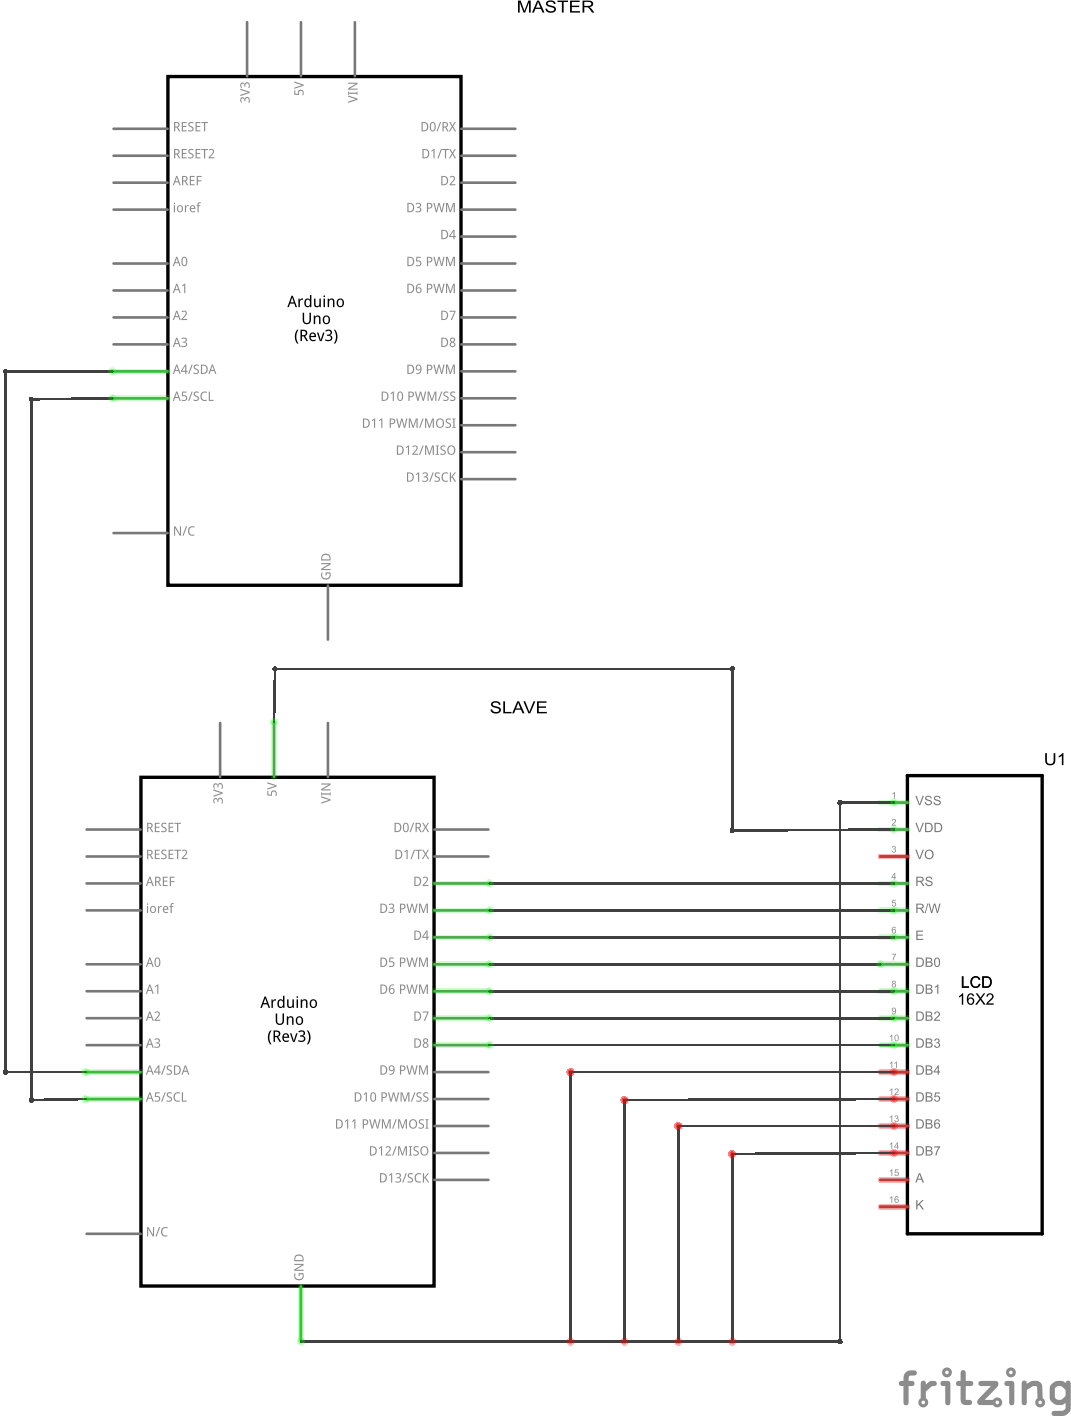
\includegraphics[width = \linewidth]{images/schem.png}
	\caption{Schematic of hardware implementation(developed using Fritzing)}
	\label{fig:schm}
\end{figure}

\subsection{Software Implementation}
See figure[\ref{fig:flow}].
\begin{figure}[!htbp]
	\centering
	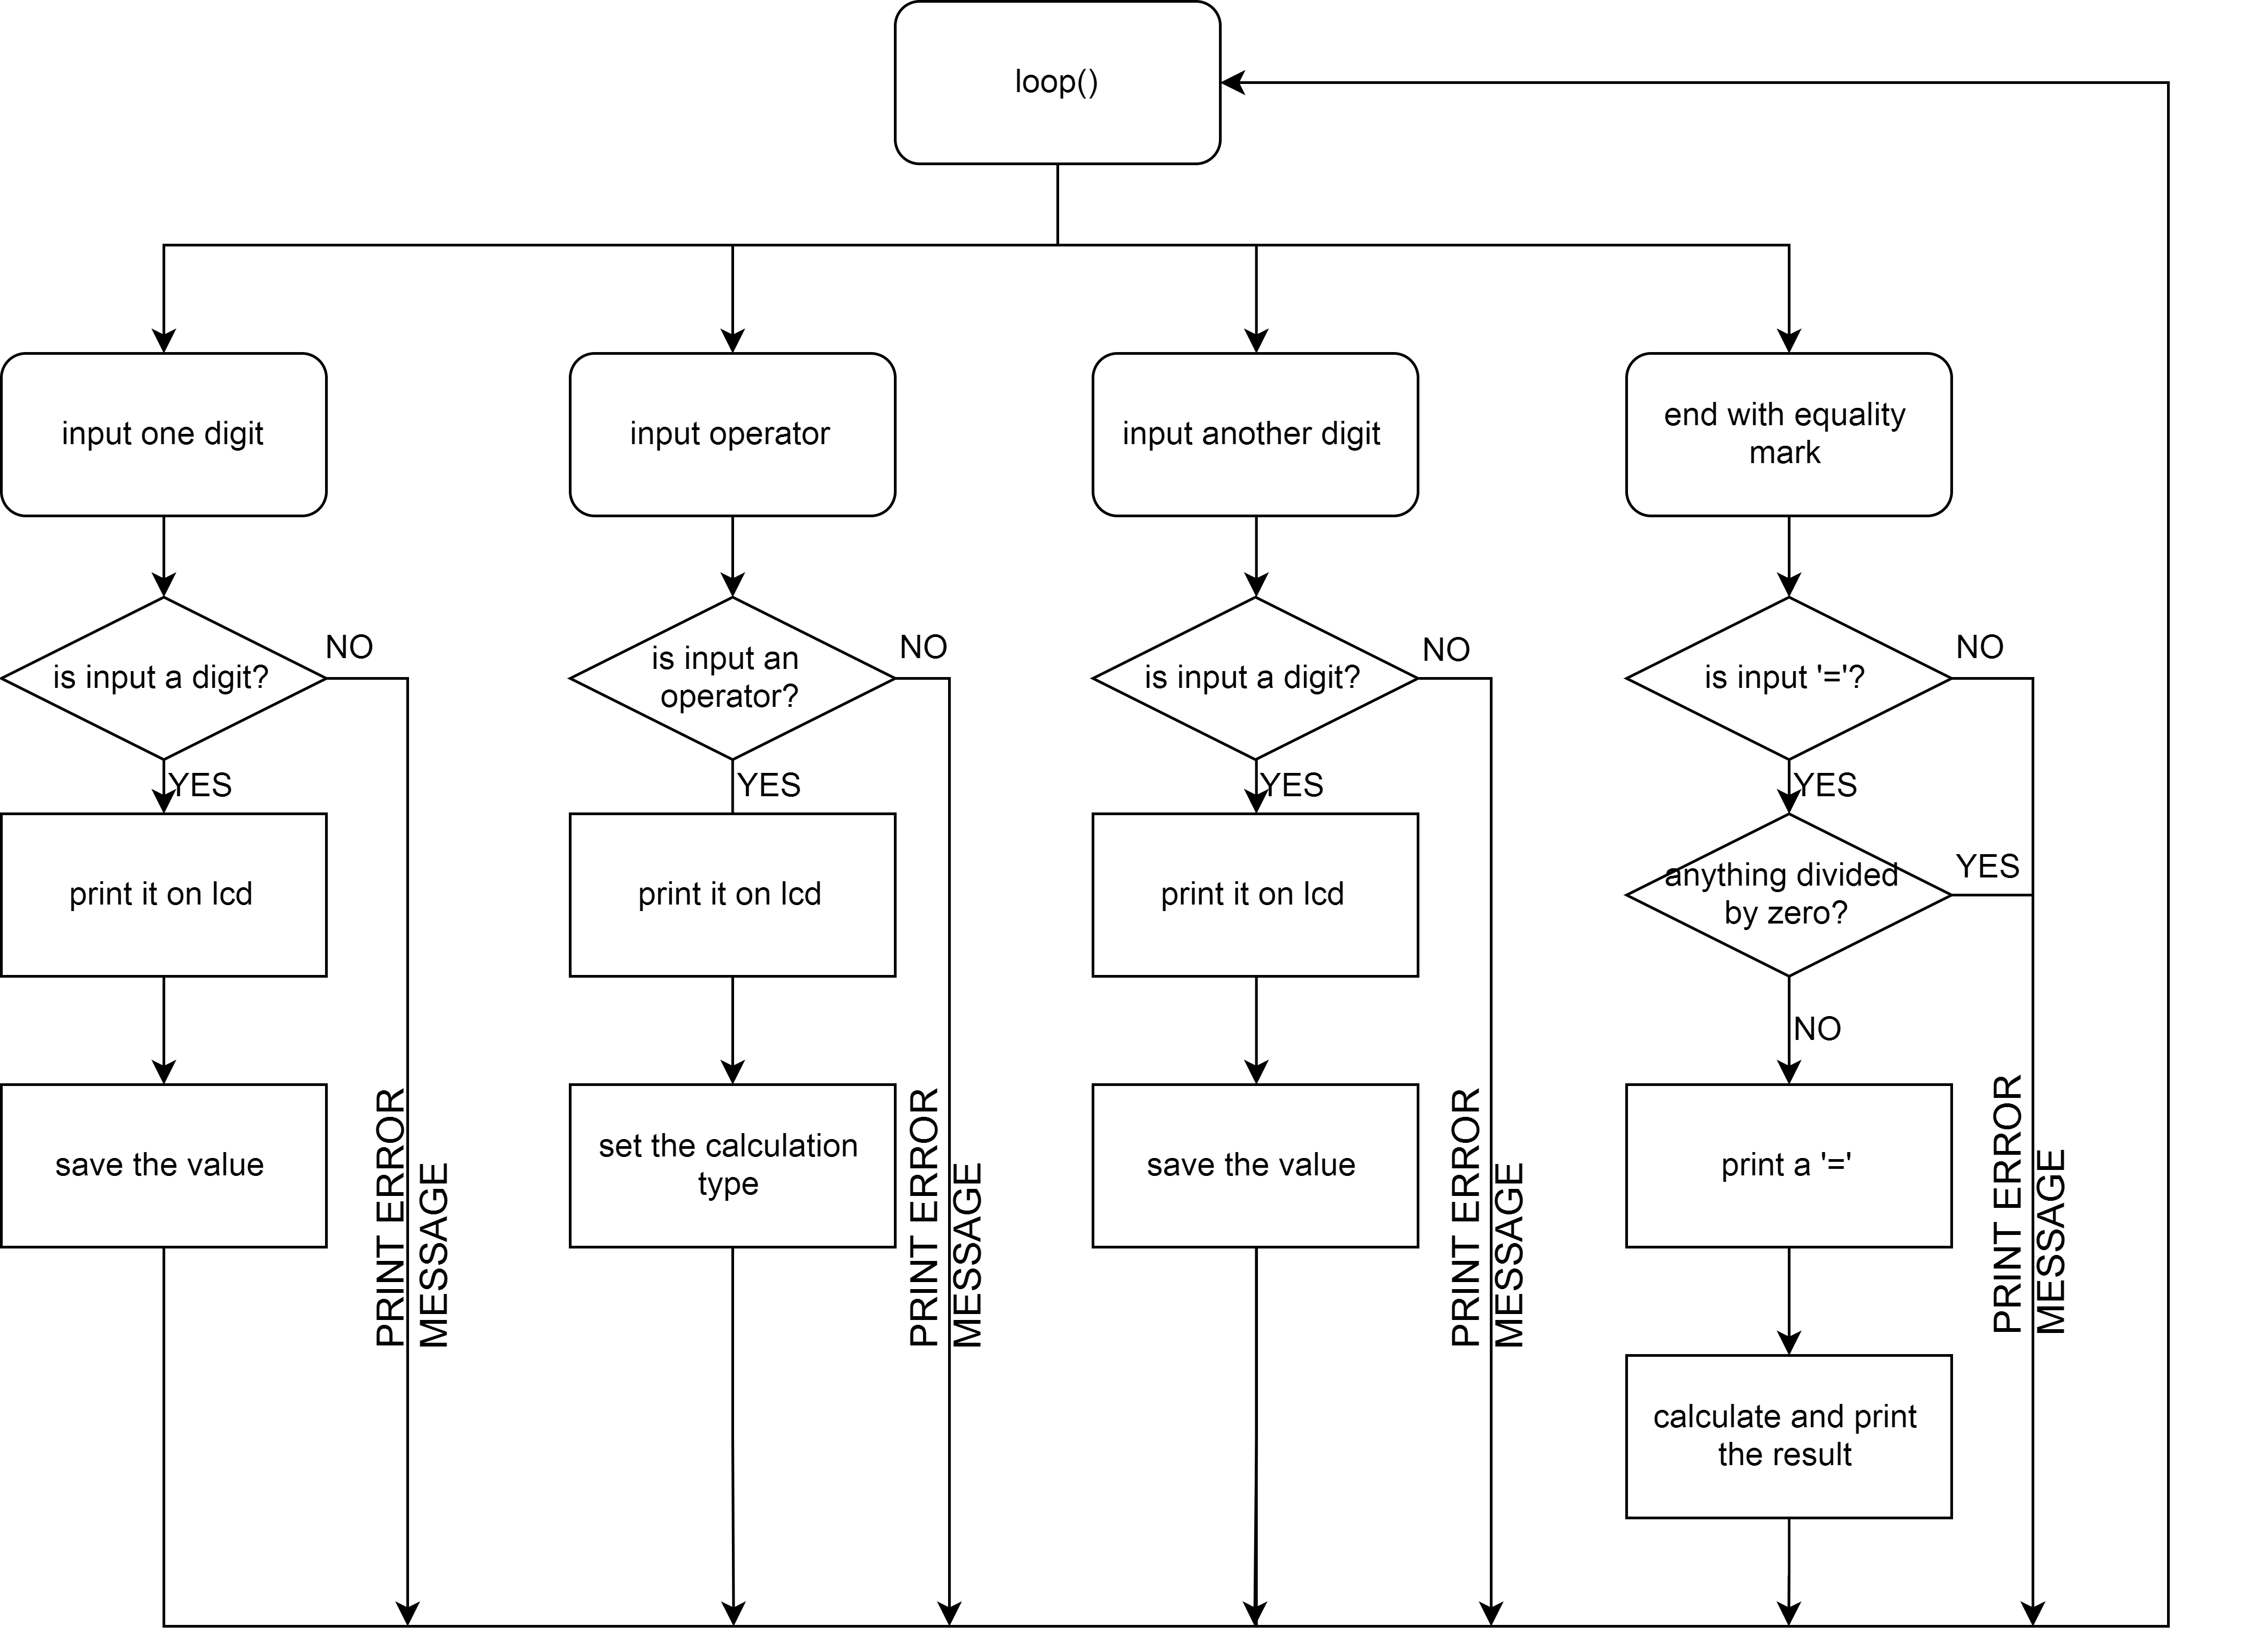
\includegraphics[width = \linewidth]{images/flow_chart.png}
	\caption{The flow of control}
	\label{fig:flow}
\end{figure}